\chapter{Metodologia}
\section{Definição das Métricas para Avaliar Eficácia dos Processamentos}
% Nesta seção, serão definidas as métricas específicas que serão utilizadas para avaliar a eficácia dos processamentos de imagem no estudo.

O fluxograma apresentado na Figura \ref{fig:fluxograma_metodologia} descreve o processo de desenvolvimento de uma metodologia para o processamento de imagens. Inicialmente, define-se e desenvolve-se os processamentos necessários, ajustando seus parâmetros e combinando-os para otimizar os resultados. Com isso, são avaliadas as métricas de desempenho para verificar a eficácia das abordagens adotadas. Se os resultados forem satisfatórios, os melhores processamentos são selecionados e o processo é finalizado. Caso contrário, analisa-se o número de tentativas realizadas: se muitas tentativas falhas ocorreram, o processamento é descartado e novas abordagens são consideradas. Se o número de tentativas ainda for baixo, o processo retorna à etapa de ajuste de parâmetros, permitindo novas tentativas até atingir os resultados desejados.

\begin{figure}[H]
    \centering
    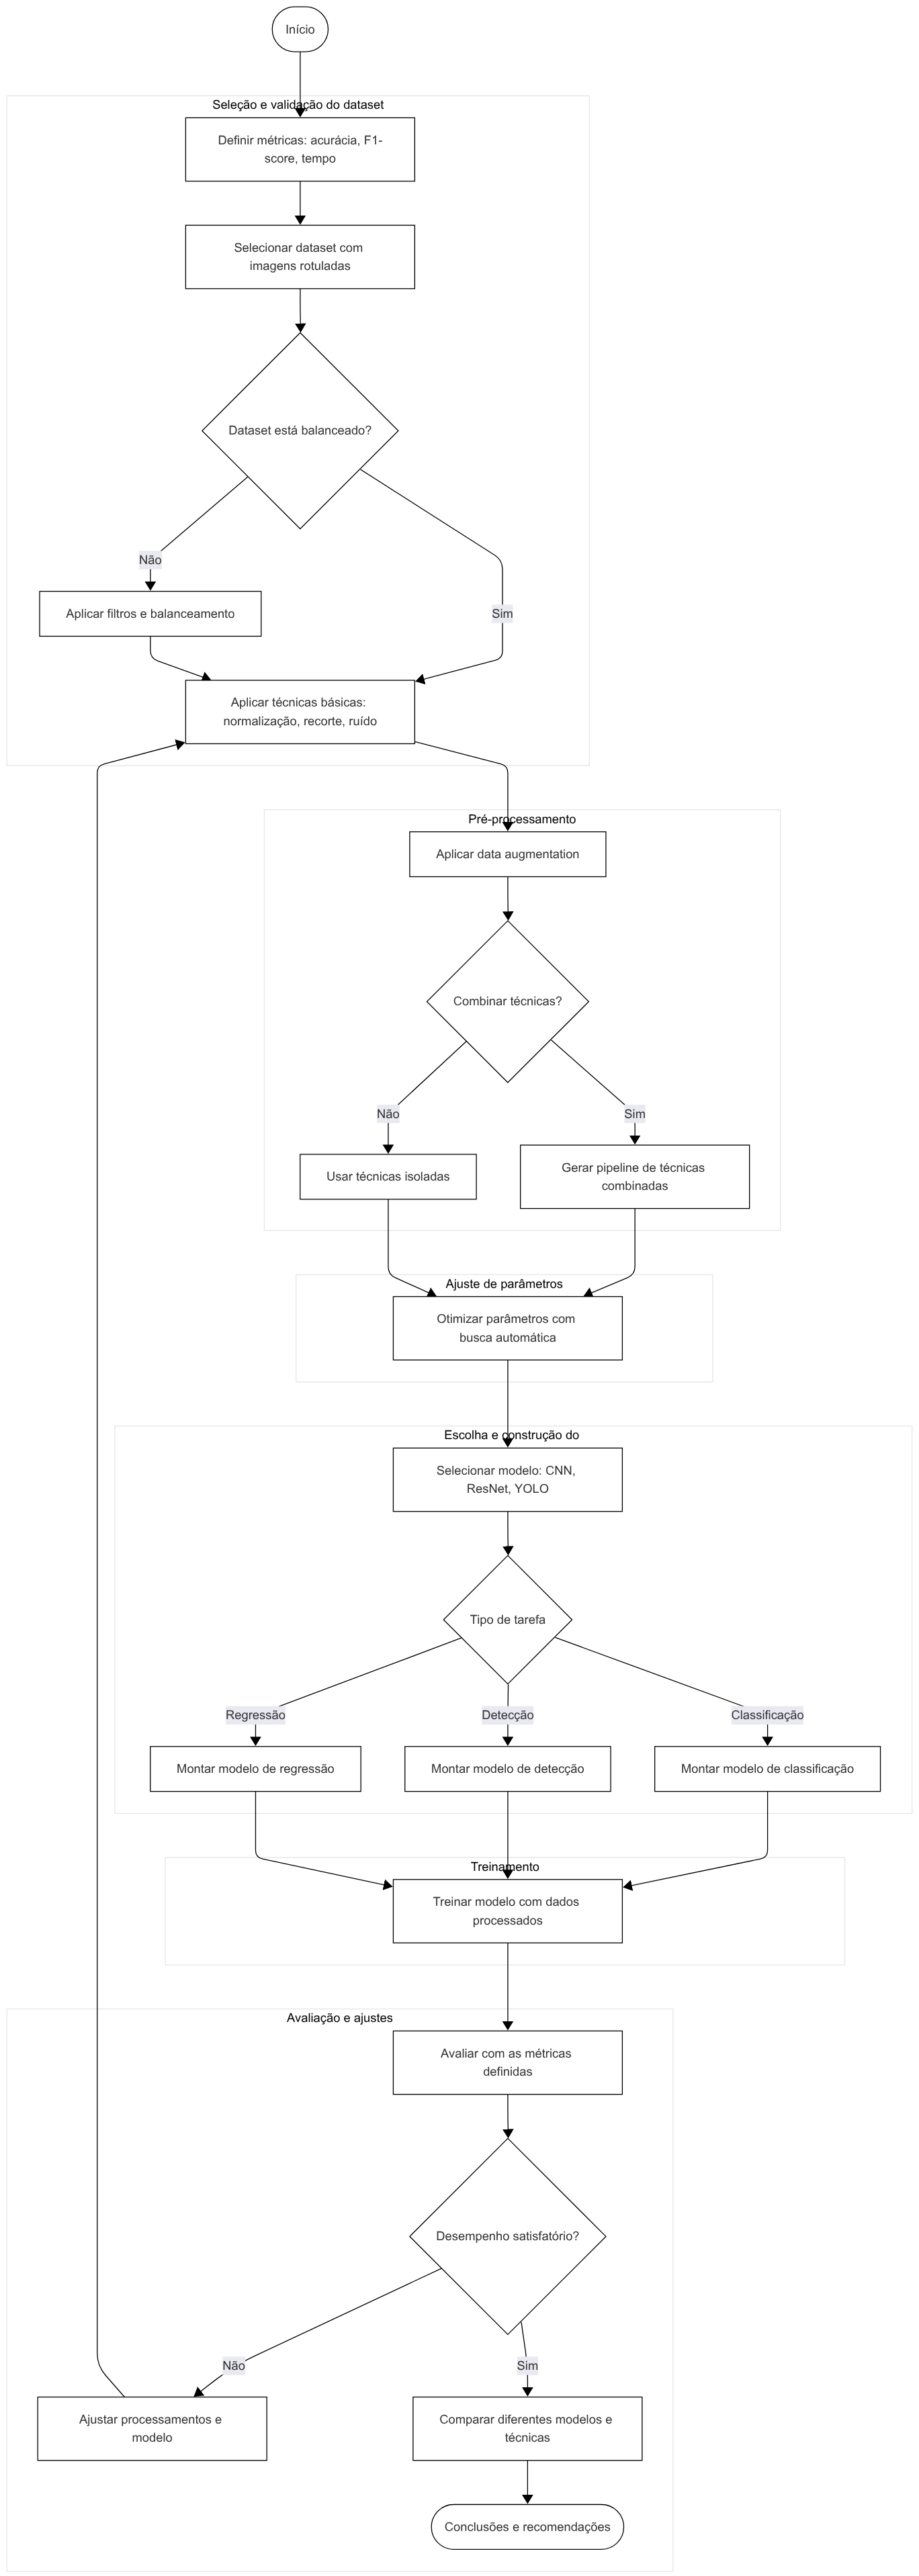
\includegraphics[width=0.7\textwidth]{img/metodologia.png}
    \caption{Fluxograma da metodologia de processamento de imagens}
    \label{fig:fluxograma_metodologia}
\end{figure}

\section{Escolha do Tipo de Modelo de Rede Neural}
Será discutida a escolha do tipo de modelo de rede neural mais adequado para as tarefas de classificação, detecção e regressão no contexto do estudo.

\section{Seleção dos Datasets para Avaliação}
Serão apresentados os critérios e a seleção dos datasets que serão utilizados para a avaliação dos processamentos de imagem.

\section{Metodologia para Combinação de Processamentos Unitários}
Aqui, será detalhada a metodologia desenvolvida para combinar diferentes processamentos unitários de imagem visando a melhoria dos resultados.

\section{Implementação de um Método de Ajuste Automático de Parâmetros}
Será descrito o método implementado para ajuste automático de parâmetros das técnicas de processamento de imagem, com o objetivo de otimização sem intervenção manual extensa.

\section{Construção de Redes Neurais para Avaliação dos Processamentos}
Nesta seção, será detalhada a construção dos modelos de redes neurais utilizados para avaliar os processamentos de imagem.

\section{Testes com Diferentes Arquiteturas e Análise de Variações nos Resultados}
Serão apresentados os testes realizados com diferentes arquiteturas de redes neurais e a análise das variações nos resultados obtidos.
